\documentclass[]{standalone}

\usepackage{graphicx}
\usepackage[linesnumbered,ruled,vlined]{algorithm2e}
\usepackage{color,soul}
\usepackage[utf8]{inputenc}
\usepackage[T1]{fontenc}
\usepackage{textcomp}
\usepackage{amsmath, amssymb}
\usepackage{caption}
\usepackage{listings}

% figure support
\usepackage{tikz}
\usetikzlibrary{calc}
\usepackage{import}
\usepackage{xifthen}
\pdfminorversion=7
\usepackage{pdfpages}
\usepackage{transparent}
\usepackage[hidelinks]{hyperref}

\pdfsuppresswarningpagegroup=1

\begin{document}
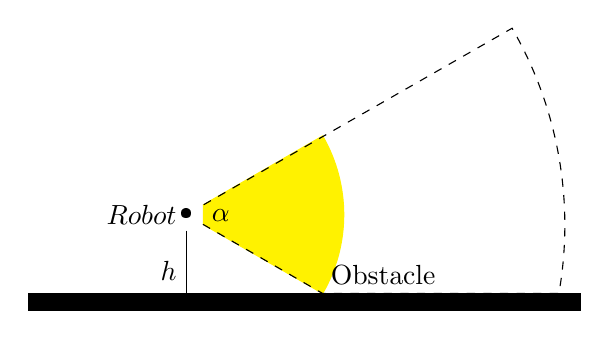
\begin{tikzpicture}[>=stealth]
	\node[] (Robot) at (0,1.01) {\textbullet};
	\node[left] (Label) at (Robot) {$Robot$};
	\filldraw[yellow] (Robot)--($(Robot)+(-30:2)$) arc (-30:30:2) -- (Robot);
	\filldraw[thick] (-2,0) -- (5,0) -- ++(0,-0.2) -- ++(-7,0) -- cycle ;
	\node[above] (wall) at (2.5,0) {Obstacle};
	\draw[dashed] (Robot)--($(Robot)+(-30:2)$) -- ++(3,0) arc (-10:30:5)--(Robot);
	\draw[] (Robot) -- ++(0,-1);
	\node[right] (a) at (0.2,1) {$\alpha $};
	\node[left] (d) at (0,0.3) {$h$};
\end{tikzpicture}
\end{document}

